\documentclass[main]{subfiles} 


\graphicspath{{img/}}


\begin{document}

\section{Implementation}
The whole project can be found in a repository on Github.
There the README will provide the necessary information regarding the implementation of the
scraper as well as how to use the interface.
All of the files were written and run in python version $3.9.12$.
Below a list of all the packages plus their respective versions that were used can be found.

\begin{itemize}
    \item \pkg[Scrapy] -  version $2.6.1$
    \item \pkg[Selenium] - version $4.1.5$
    \item \pkg[Webdriver\_manager] - version $3.5.4$
    \item \pkg[Numpy] -  version $1.22.3$
    \item \pkg[Pandas]  - version $1.4.2$
    \item \pkg[Time]
    \item \pkg[Datetime]
    \item \pkg[Openpyxl] - version $3.0.9$
    \item \pkg[Tk (tkinter)] - version $0.1.0$
    \item \pkg[Pillow] - version $9.1.1$
\end{itemize}

\subsection{Structure of the project}

\begin{forest}
  for tree={
    font=\ttfamily,
    grow'=0,
    child anchor=west,
    parent anchor=south,
    anchor=west,
    calign=first,
    edge path={
      \noexpand\path [draw, \forestoption{edge}]
      (!u.south west) +(7.5pt,0) |- node[fill,inner sep=1.25pt] {} (.child anchor)\forestoption{edge label};
    },
    before typesetting nodes={
      if n=1
        {insert before={[,phantom]}}
        {}
    },
    fit=band,
    before computing xy={l=15pt},
  }
[/.
    [comparis\_webscraper
        [comparis\_webscraper
            [spiders
                [comparis\_scraper.py]
                [property\_code\_scraper.py]
            ]
            [items.py]
            [middlewares.py]
            [pipelines.py]
            [settings.py]
        ]
        [scrapy.cfg]
    ]
    [data
        [database.xlsx]
        [property\_codes.csv]
        [property\_details.csv]
    ]
    [GUI
        [cleaning\_database.py]
        [zoes\_version\_1.py]
        [zoes\_version\_2.py]
        [zoes\_version\_3.py]
        [zoes\_version\_4.py]
    ]
    [README.md]
    [Makefile]
    [.gitignore]
    [.git]
]
\end{forest}

\subsection{Implementation of the Web Scraper}
As mentioned previously, the web scraping was done by utilizing two different tools, \pkg[Scrapy] and \pkg[Selenium].
When programming the spider, the main challenge was to implement the vision of what it should do.

When called, the spider should do the following:
\begin{enumerate}
    \item Activate the browser via \hspace*{-6pt} \pkg[Selenium]
    \item Access a list of predefined \acsp*{url}
    \item Loop through every \acs*{url} and activate the \js
    \item Download $22$ datapoints from several locations on the website
    \begin{itemize}
        \item If not available, no value was returned
    \end{itemize}
    \item Process the data via the input processor of the \hspace*{-6pt}\pkg[ItemLoader]
    \item Store data in the \hspace*{-6pt} \pkg[ItemLoader] until the loop has finished
    \item Output (yield) the data from the \hspace*{-5pt} \pkg[ItemLoader] into the "data" directory as \hspace*{-5pt}
    \pkg[.csv] file with the download date in the name
\end{enumerate}

\subsubsection{Obtaining the List of \acsp*{url}}
Web scraping turned out to be a mix of close investigation of \acs*{html} source codes, 
creative problem solving and a lot of trial and error. 
Obtaining all the property \acsp*{url} was a clear example of this.

Although on a smaller scale, 
it also required a combination of \pkg[Scrapy] and \pkg[Selenium] in order to trigger the \js's.

When a user runs a search on Comparis (e.g. house for purchase in a specific location), 
the website will filter through all the listings and return the corresponding properties.
If the user triggers the \js by scrolling, Comparis will load a \acs*{json} 
containing the unique ID's of \textbf{all} search results at the bottom of their \acs*{html}.
This can be seen when right clicking on the page and selecting "Inspect" and entering \pkg[\_\_NEXT\_DATA\_\_] 
in the search field.

\begin{figure}[htbp]
    \centerline{
        
\includegraphics[width = 60mm]{prog_3.png}}
    \caption{Inspect Elements on Browser}
    \label{fig:listing}
\end{figure}

From there on, \pkg[Selenium] will pass the "current state" (i.e. state of \acs*{html} after \js manipulation)
to the spider for the analysis.
The spider then yields the ID's and creates \acsp*{url} by adding them to the end of the path component of the \acs*{url}
(which is how Comparis refers to their detail pages). 

\begin{figure}[htbp]
    \centerline{
        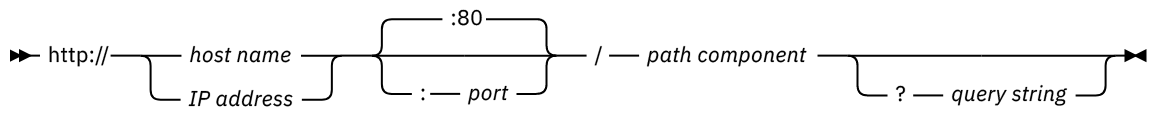
\includegraphics[width = 80mm]{prog_4.png}}
    \caption{Structure of a \acs*{url}}
    \label{fig:listing}
\end{figure}

\subsubsection{Creating the "property-scraper" Spider}






\subsection{Implementation of the \ac{gui}}

\subsubsection{Organizing the scraped data}
The first step to building the \ac{gui} is organizing the data that we obtain from the web scraping.
We first analyze the dataset and then clean it for the GUI to function correctly.
This is done in the program \pkg[cleaning\_database.py] which we also use to do the data analysis in our parallel project. \par
In this cleaning program, we first load the dataset. 
Then we print the headings and the description to check the data and the types.
We remove variables that are misspelled, incorrect or missing. 
We then proceed to split the address from the zip code, to get the zip code in a separate column. 
We do this as we want to be able to search properties within a certain zip code. 
Finally we save the dataset. This dataset is the one that the GUI will use to return information to the user.

\subsubsection{Building the \ac{gui}}

To build the \ac{gui} we created a new program named main4.py.
We first defined what we wanted our \ac{gui} to do. 
We decided, we wanted the user to be able to search for a property within a certain price range, 
or with a specific number of rooms or within a specific zip code. 
Thefore to build this \ac{gui} we needed to have different tabs to search for these separately.
We also needed to be able to clear the search to be able to run the program multiple times. \par
In the program we start by defining the characteristics of the root widget otherwise known the main window,
such as height, width and title. We then add the notebook instance to add tabs to the interface.
These are known as frames in tkinter. From there, we format the frames and add the labels and entries we wish to have in each tab. 
We then add the scrollbar to the root window to be able to scroll through the returned properties if the list is long. 
We also add a treeview instance so that the pulled data from the dataset is displayed in hierarchical and tabular structure. 
Finally we define the fuctions that retrieve the data from the database to the interface. 
We also add a function to clear the searched information and start anew. \par
This is a very basic \ac{gui} to make it easier for the user to interact with the scraped data.
The aim would be to develop the interface searches that are more complex, such as conditional searches with more than one characteristic.

\begin{tikzpicture}[auto, node distance = 4mm and 6mm, start chain = going below]
    \begin{scope}[nodes={on chain, join=by line}]
        \node[startstop] (start) {Start};
        \node[input] (in1) {Load Scraped data};
        \node[decision] (dec1) {Is Data Cleaned?};
        \node[input] (in2) {Start GUI by importing tkinter};
        \node[process] (pro2a) {link to cleaned dataset};
        \node[process] (pro2) {Format main window};
        \node[process] (pro3) {Format frames as tabs};
        \node[process] (pro4b) {Create functions for each tab};
        \node[process] (pro5) {Define main loop};
        \node[decision] (dec2) {Check GUI is working};
        \node[input] (in3) {User can serch properties};
        \node[decision] (dec4) {End the program};
        \node[startstop] (start1) {End};
        %%%%%%%%%%%%%
    \end{scope}
    \begin{scope}
        \node[process, left=of dec1] (pro1) {Clean and Organize data};
        \node[process, left=of dec2] (pro6) {Find bug};
        \node[process, left=of dec4] (pro7) {Re-run the program};
        \draw [->] (dec1) |- (pro1); %{No} missing
        \draw [->] (dec2) |-  (pro6); %{No} missing
        \draw [->] (dec4) |-   (pro7); %{No} missing
        \draw [->] (pro1) |- (pro2);
        \draw [->] (pro6) |-  (in2);
        \draw [->] (pro7) |-  (in3);
    \end{scope}
\end{tikzpicture}

\subsection{Maps?}

\end{document}